% !TEX root = ../../main.tex

\chapter{Cost Estimation}

\label{chapter:cost-estimation}
In this chapter, we share the results of our experiments and explain they are used for constructing four different cost models. The \hyperref[sec:5-motivation]{first section} shows the results of the runtime experiments, motivating why a cost model is necessary. In the \hyperref[sec:5-gpu-performance-analysis]{next section} the collected profiling metrics are aggregated and analysed, giving insight into how GPU intrinsics can affect the trade-off. \autoref{sec:5-feature-engineering} details the process of aggregating and enriching our results to generate an appropriate dataset for the estimators to train on. In \autoref{sec:5-cost-models}, we talk about how we used the enriched results, from the runtime and profiling experiments, to create multiple cost models. Each model is made for a specific purpose and offers different ways to solve the problem.

\section{Motivation}
\label{sec:5-motivation}
This section shows why there is a need for accurate cost estimation for choosing between factorization and materialization. We motivate in three stages. First the benefit of factorization is shown, second we show the impact of data \& model characteristics. By visualizing the performance ratio ($\frac{\text{Time}_M}{\text{Time}_F}$) against a range of independent variables we uncover the first trends that influence the F/M trade-off. Last, we show why GPUs are important  to consider. All figures and values in this section are created with the data collected with the experiments on synthetic datasets, unless specified otherwise.

\subsection{Benefit of factorization}
\begin{figure}[ht]
    \centering
    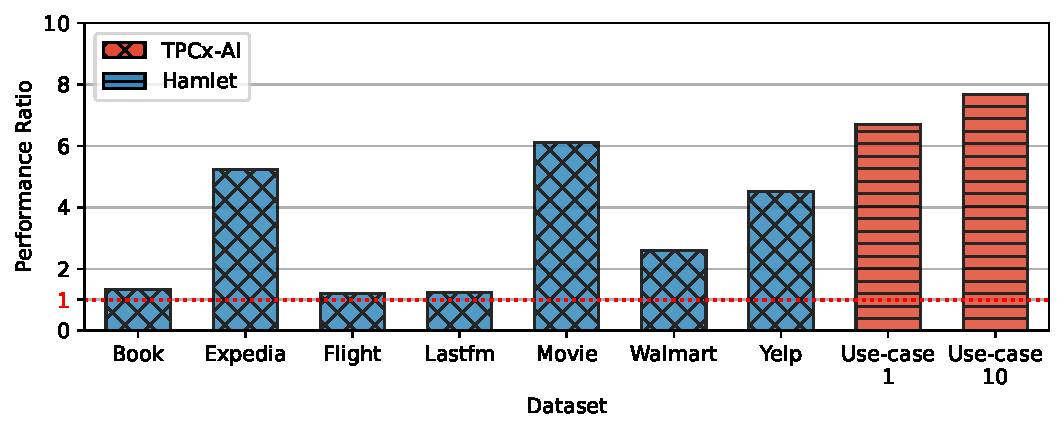
\includegraphics[width=0.7\linewidth]{chapters/05_cost_estimation/figures/real_datasets_speedup.pdf}
    \vspace*{-5mm}
    \caption[Performance gain with factorization on real datasets]{Average Performance ratio of ML models for positive cases ($\text{Time}_M > \text{Time}_F$), split per tested real dataset.}
    \label{fig:5-real-perf-ratio}
\end{figure}

The goal of factorized ML is reducing the number of redundant operations performed during training of a model, to make this process more efficient, i.e., faster. We show the performance gain of factorization over materialization, on real datasets, in \autoref{fig:5-real-perf-ratio}. Exploring factorization is beneficial, as for those cases where it is faster (which is $18\%$ of the tested cases on real datasets), the average speedup is $5.1\times$. In the most extreme cases the training time is reduced by more than $20$ seconds, a reduction by a factor of $27$. In scenarios where training happens frequently, e.g., during hyperparameter optimization or online learning, this can lead to significant time savings.

% We group the Data and Model characteristics as they both influence the actual computations being executed. The hardware characteristics influence how these computations are carried out on the hardware and are discussed separately. 

\subsection{Data \& Model Characteristics}
\begin{figure}[ht]
    \centering
    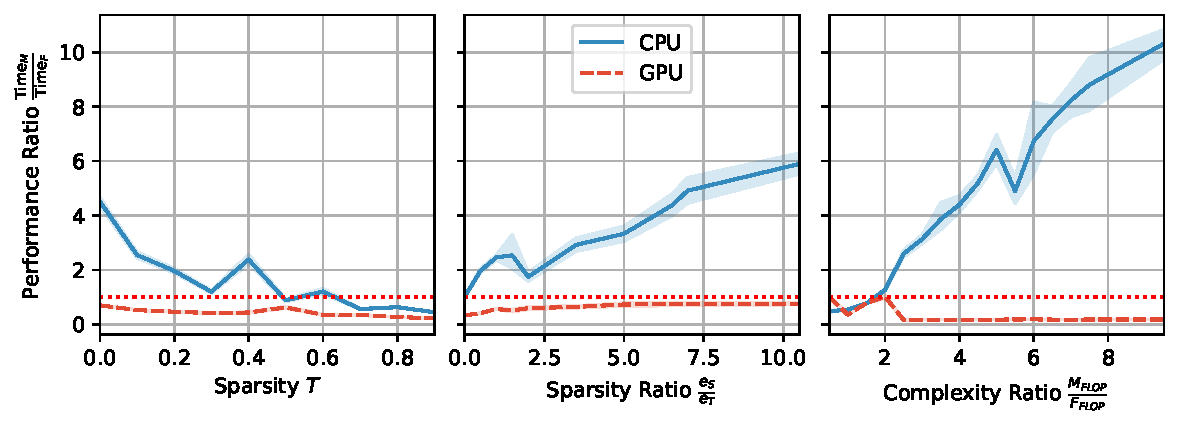
\includegraphics[width=\linewidth]{chapters/05_cost_estimation/figures/motivation_perf_ratio_vs_data_chars.pdf}
    \caption[Performance ratio for various data characteristics]{Performance ratio against various data characteristics. Broken down by compute type (CPU/GPU). $99\%$ confidence interval shown as shaded area. The sparsity ratio is defined as the sparsity of the source tables $S_k, k\in[1,n]$ divided by the sparsity of target table $T$. Sparsity of $S$ is defined as the total non-zero values in the base tables divided by the total number of cells in the base tables, $\frac{\sum_{k=1}^{n} nnz(S_k)}{\sum_{k=1}^{n} r_{S_k} \times c_{S_k}}$. High sparsity ratio means the target table is relatively denser than the source tables.}
    \label{fig:5-complexity-ratio-vs-data-chars}
\end{figure}
We show the impact of various data characteristics on the performance ratio in \autoref{fig:5-complexity-ratio-vs-data-chars}. The figure shows a slight negative correlation between performance ratio and sparsity of target table $T$. The second column shows more insight into the relation between performance and sparsity. It shows that when the sparsity ratio is low, i.e., compared to the base tables $S_k$, $T$ has more zero values, factorization is likely slower than materialization. The right-most plots show that a higher complexity ratio ($\frac{FLOP_M}{FLOP_F}$) is likely to lead to factorization being the preferred training method. This is in line with the intuition that factorization is beneficial when it saves redundant computations.

Important to note is that the correlation between these data characteristics and the speedup factorization brings is not as clear when using GPUs for computation. This is due to the fact that the computations are not compute-bound, but memory-bound. This view is discussed thoroughly in \autoref{sec:5-gpu-performance-analysis}, where the metrics, collected in the profiling experiments, are analysed.


\subsection{Hardware Characteristics}
\begin{figure}[ht]
    \centering
    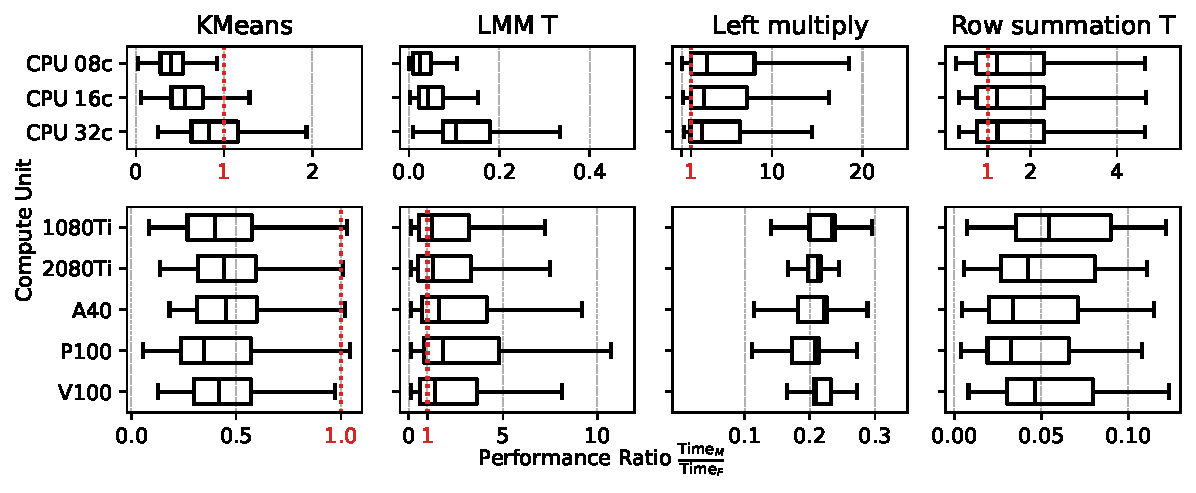
\includegraphics[width=\linewidth]{chapters/05_cost_estimation/figures/motivation_speedup_per_operator_per_gpu.pdf}
    \caption[Performance ratio plotted against hardware]{Performance ratio, of various operators on synthetic data, against hardware. The performance ratio is shown to be affected by hardware choice.}
    \label{fig:5-gpu-characteristics}
\end{figure}
The hardware used for computation impacts the runtime of a program, but here we show it also impacts the F/M trade-off. Different compute unites (i.e., CPU or GPU type) have a different decision boundary for when to use factorization over materialization. This is shown in \autoref{fig:5-gpu-characteristics}. Differing hardware impacts the performance ratio differently per operator. For example, the (mean$\pm$std.) performance ratio of transposed Left Matrix Multiplication on the P100 is $3.03\pm2.70$, while on the V100 it is slightly lower with $2.32\pm2.21$. But, for Left (scalar) multiplication the V100 has the higher performance ratio of $0.21\pm0.04$, against the P100's lower $0.19\pm0.05$.

\begin{table}[ht]
    \centering
    % LTeX: enabled=false
\begin{tabular}{lrrrr}
\toprule
Compute Unit & Mean & Std. Dev. & Count & \% with Speedup \\
\midrule\midrule
CPU 08c & 1.27 & 0.25 & 172 & 1.78\% \\
CPU 16c & 1.32 & 0.34 & 579 & 5.99\% \\
CPU 32c & 1.48 & 0.46 & 2873 & 29.74\% \\
1080Ti & 2.27 & 1.60 & 432 & 4.47\% \\
2080Ti & 1.87 & 1.09 & 425 & 4.40\% \\
A40 & 2.00 & 1.20 & 392 & 4.06\% \\
P100 & 2.52 & 1.84 & 461 & 4.77\% \\
V100 & 1.95 & 1.13 & 404 & 4.18\% \\
\bottomrule
\end{tabular}

    \caption[Performance ratio of ML models for cases where factorization has positive impact.]{Mean performance ratio of ML models for cases where factorization is preferred over Materialization (speedup > 1). This shows hardware choice is a large factor in when to choose factorization over Materialization.}
    \label{tab:5-speedup-per-gpu}
\end{table}

For cases where factorization is preferred over materialization ($\text{Time}_M > \text{Time}_F$), there are differences between the GPUs. Both the mean performance ratio, and the count of cases where F is faster than M varies, as shown in \autoref{tab:5-speedup-per-gpu}. This shows that the choice of hardware is a factor in when to choose factorization over materialization. However, the difference between GPU types is not as large as the difference between CPU and GPU. Therefore, it is more interesting to treat the compute-type as a separate feature in the cost models, and not necessarily the specific GPU type.

Another interesting observation can be seen when comparing the performance ratio against the complexity ratio \cite{schijndel_cost_estimation}, for different hardware settings. As explained in \autoref{sec:3-cost-estimation-for-factorized-ml} the complexity is defined as the number of FLOPs needed to perform an operation. The ratio is defined as the complexity of the factorized case divided by the complexity of the materialized case. Thus, per \cite{schijndel_cost_estimation}, the higher this ratio the more beneficial it is to use factorization. However, our experiments show that while this is the case for a lot of operators on CPU, when performing the computations on GPUs this is not always the case. This is shown in \autoref{fig:5-complexity-ratio-vs-performance-ratio}. The next section explores why this is the case.

\begin{figure}[ht]
    \centering
    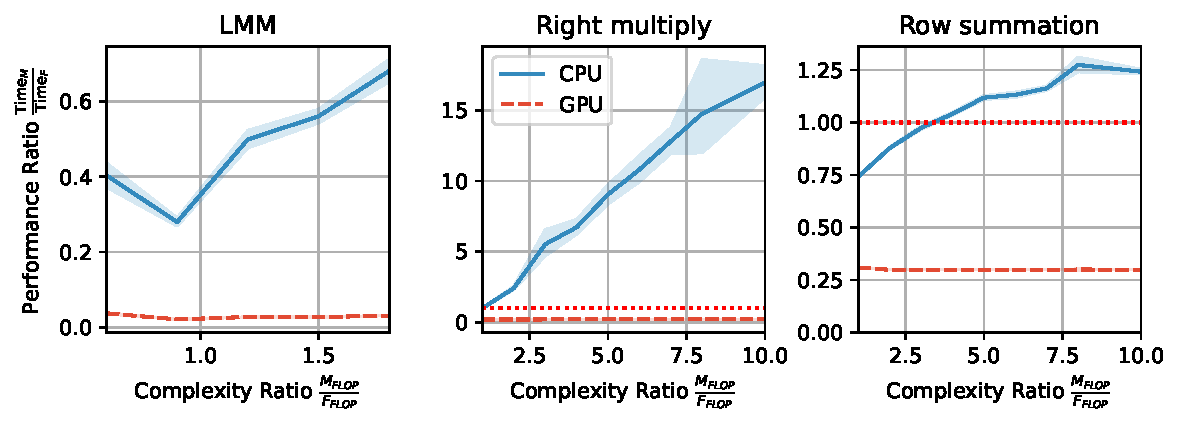
\includegraphics[width=\linewidth]{chapters/05_cost_estimation/figures/motivation_speedup_complexity_ratio.pdf}
    \caption[Performance ratio plotted against complexity ratio]{Performance ratio, of various operators on synthetic data, against complexity ratio, broken down by CPU and GPU. 95\% Confidence interval shown as shaded area. Where a lot of operators show clear correlation between the complexity ratio and the performance ratio on CPU, this is not the case for GPU.}
    \label{fig:5-complexity-ratio-vs-performance-ratio}
\end{figure}


\section{GPU Performance Analysis}
\label{sec:5-gpu-performance-analysis}
A preliminary step for creating an accurate cost model is to understand the performance characteristics of scenarios we are testing. This section analyses the profiling metrics collected during the experiments, to understand how the choice of hardware impacts the trade-off between factorization and materialization. The first analysis is to compare the memory cost and math cost of the profiled scenarios. Per NVIDIA, a fitting way to estimate the runtime of a GPU program is to compute $max(T_{mem}, T_{math})$. In this formula $T_{mem}$ is the time it takes to transfer data to and from GPU memory, and $T_{math}$ is the time it takes to perform the actual computations. This is in line with the highly parallel nature of GPUs. If data cannot be transferred to the GPU fast enough the GPUs Streaming Multiprocessors will be idle, waiting for data. If this is the case, the program is memory-bound. In the opposite case, where $T_{math} > T_{mem}$, the program is compute-bound. In this section we show which is the case for our experiments, and how we can use this to estimate the runtime of an ML training scenario.

\begin{figure}[ht]
    \centering
    \begin{minipage}{0.50\textwidth}
        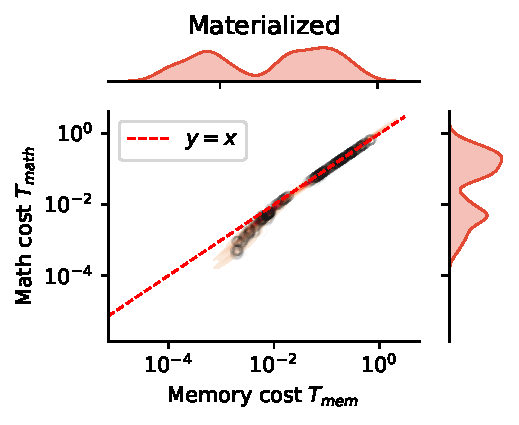
\includegraphics[width=\linewidth]{chapters/05_cost_estimation/figures/profiling-mem-vs-compute-materialized.pdf}
    \end{minipage}\hfill
    \begin{minipage}{0.50\textwidth}
        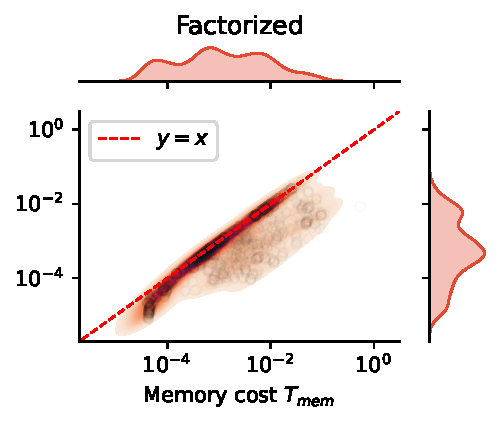
\includegraphics[width=\linewidth]{chapters/05_cost_estimation/figures/profiling-mem-vs-compute-factorized.pdf}
    \end{minipage}
    \caption[Memory cost vs math cost of profiled scenarios]{Memory cost ($T_{mem}$) vs compute cost ($T_{math}$) of profiled scenarios. The memory cost is computed as the total number of bytes read and written to memory divided by the measured average memory bandwidth. The math cost is the number of cycles the Streaming Multiprocessors were active divided by the measured average SM frequency.}
    \label{fig:5-profiling-mem-vs-compute}
\end{figure}

\autoref{fig:5-profiling-mem-vs-compute} shows the distribution of $T_{mem}$ vs. $T_{math}$. As expected, these values are highly correlated ($\rho = 0.99$). Almost none of the profiled scenarios have a higher math cost than memory cost (points are below the $y=x$ line). This shows that the computations are memory-bound, and that predicting the memory cost should be the focus of our cost estimation. The difference between factorization and materialization is also substantial. This first becomes obvious when calculating the correlation, for the materialized cases $\rho = 0.99$, for the factorized cases this is only $0.40$. The cause for this is that with the materialized case the GPU only has to handle a single matrix (or two matrices in the case of matrix multiplication). The normalized matrix used for the factorized case consists of more separate matrices ($S_k,I_k,M_k, k \in \{1 \ldots n\}$), each used in different computations. On average, this reduces both the memory and compute cost. However, it also causes a shift away from the $T_{mem} = T_{math}$ line, as the computations on the different matrices are executed in sequence on the GPU.

\begin{figure}
    \centering
    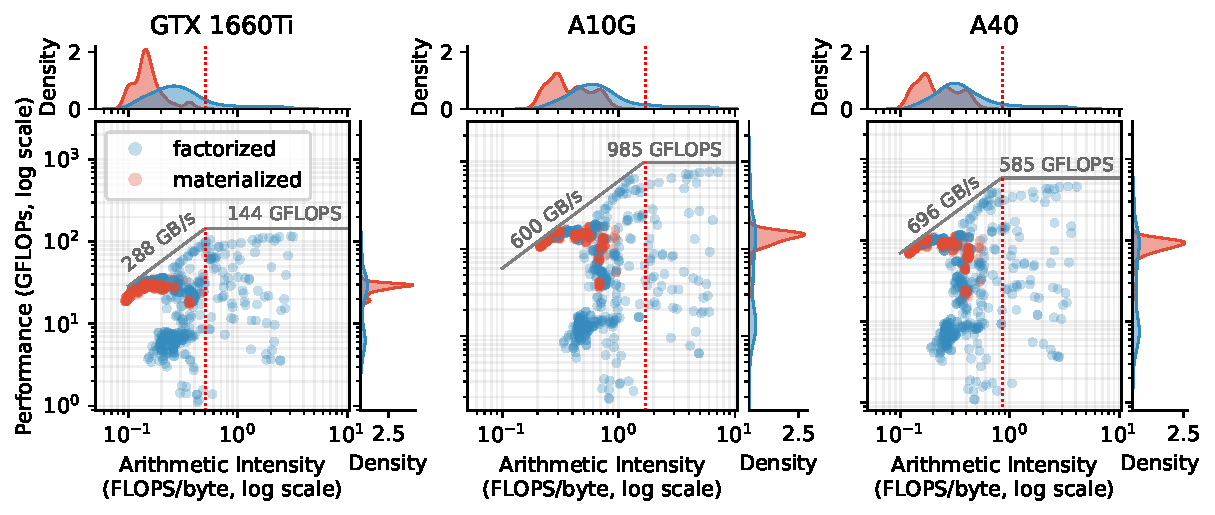
\includegraphics[width=\linewidth]{chapters/05_cost_estimation/figures/roofline-plot.pdf}
    \caption[Roofline chart comparing F/M, per GPU]{Roofline chart showing where the performance of the GPUs lies in the memory-bound vs compute-bound spectrum. The subplots on top and right side of each figure show the distribution along the performance (GFLOPs) and operational intensity (FLOPS/byte) axes. Similar GPU types have similar distributions.}
    \label{fig:5-roofline-plot}
\end{figure}

\subsubsection*{Roofline Model}
More insights into the efficiency of the tested scenarios, and the differences between factorization and materialization, and GPU types, can be gained by using a roofline model. It is a “model that offers insight insights \ldots on improving parallel software and hardware for floating point computations” \cite{roofline}. The roofline model shows whether an operator on a given scenario is memory- or compute-bound. The x-axis shows arithmetic intensity of a program in FLOPs per byte (in our case a program is an operator executed on a given dataset), the y-axis the (attainable) performance in GFLOPS. The roofline (top line in grey) shows the bound on performance of a given GPU. It is constructed by taking the maximum memory bandwidth and the maximum number of FLOPS the GPU can perform per second. The point where they meet (\textit{ridge point}) tells you the minimum arithmetic intensity needed to allow full utilization of a GPUs compute capacities. By plotting programs on such a roofline chart one can reason about whether they are compute- or memory-bound by checking whether it is to the left (memory bound) or to the right of the \textit{ridge point's} x coordinate (compute bound). This is insightful because it shows where the opportunity for optimization lies by identifying bottlenecks.

The roofline charts for the performed profiling experiments are shown in \autoref{fig:5-roofline-plot}. These charts confirm that almost all scenarios are memory-bound. But, the interesting observation from this plot is the impact of GPU type, and the difference between factorization and materialization. The differences between GPUs are most obvious in the right distribution plots. The A10G and A40 are much more powerful GPUs. On the GTX1660Ti most scenarios reach a low compute performance as they hit the memory bound. The A10G and A40, however, have a much higher memory bandwidth. Thus, the scenarios reach a higher average performance. The gap these plots show between factorization and materialization gives more valuable insights. The materialized operators have lower arithmetic complexity than their factorized equivalents (shown in the top density plots). This means that, on average, the factorized operators are less memory-bound, and thus can utilize a larger part of the GPUs compute capacity. However, the factorized operators show a much larger variance in attained performance (right density plots) due to the fact that the operations on different parts of the normalized matrix are not parallelized. These operators can likely be optimized, so they can take advantage of the GPUs compute capacity more efficiently.

\begin{figure}[ht]
    \centering
    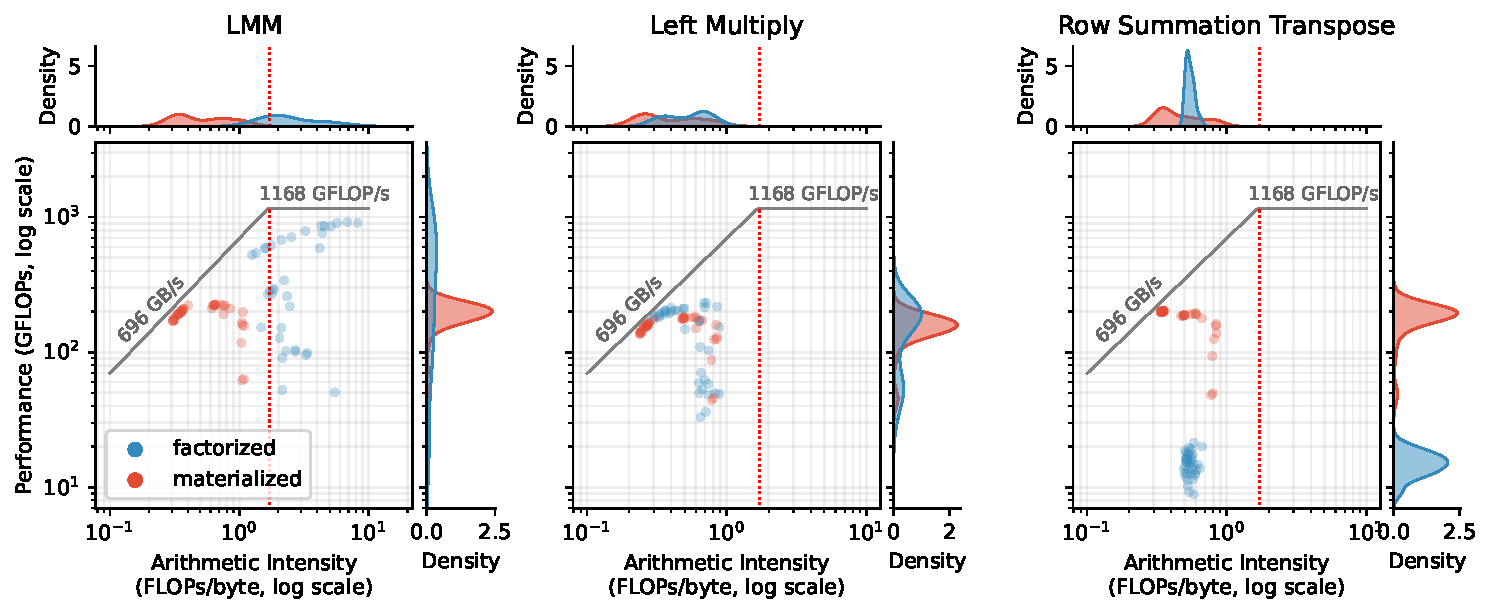
\includegraphics[width=\linewidth]{chapters/05_cost_estimation/figures/roofline-operators.pdf}
    \caption[Roofline chart per operator]{Roofline chart comparing factorization and materialization for Left Matrix Multiplication, Left Scalar Multiplication and Row Summation Transpose. Metrics from NVIDIA A40.}
    \label{fig:5-roofline-operators}
\end{figure}

A roofline chart for a selection of operators is shown in \autoref{fig:5-roofline-operators}. This breakdown per operator further shows the differences between factorization and materialization. Compared to the materialized case, the factorized case of Left Matrix Multiplication shows extremely large variance in performance, which is in line with the use of the normalized matrix explained previously. Although, overall, using factorization seems beneficial for LMM when looking at these profiling metrics (values move to the top and right, indicating higher saturation of the available resources). For Left Scalar Multiplication the gap between F and M is much smaller, which is logical as the factorized case only multiplies the Source matrices with the scalar, which is a simpler operation than the one needed for LMM. The right-most plot shows this limitation even more clearly, showing significantly less utilization of the GPU capabilities than the materialized case for Transpose Row Summation. The complete set of roofline plots broken down per operator can be found in \autoref{appendix:analysis-additional-figures}.

\section{Feature Engineering}
\label{sec:5-feature-engineering}
From our experiments (further detailed in \autoref{sec:6experiment-setup}) we have a dataset with the runtime for each scenario, defined as the combination of a dataset, operator, model type (F/M) and hardware configuration. This section details the process of preprocessing and enriching this dataset with additional features. The goal is to create a dataset that can be used to train the cost models. The features we add are based on the profiling metrics collected during the experiments, and the data and model characteristics. The process is visualized in \autoref{fig:5-feature-enrichment}. The complete feature set is described in \autoref{appendix:features}, a subset is discussed here and shown in \autoref{tab:5-feature-subset}.

\subsection{Preprocessing Profiling Metrics}
\begin{figure}[ht]
    \centering
    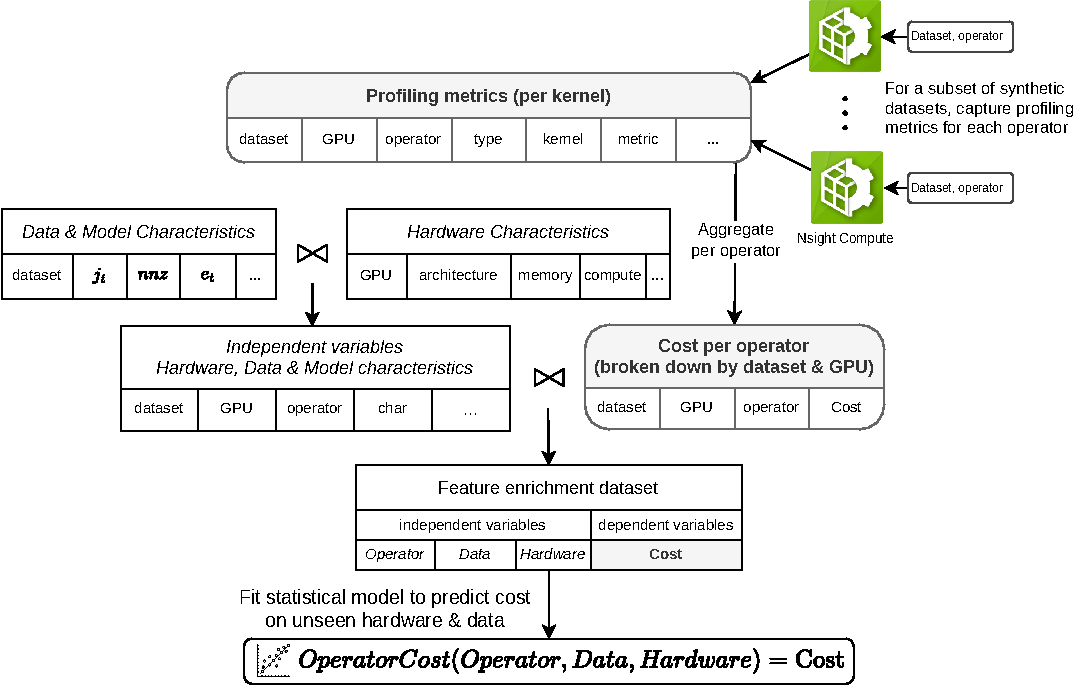
\includegraphics[width=\linewidth]{chapters/05_cost_estimation/figures/feature-engineering.pdf}
    \caption[Feature enrichment workflow]{Workflow of enriching the collected data with additional features from the profiling experiments. Items related to these profiling experiments are \textbf{bolded}, while the features from the data, model \& hardware characteristics are \textit{italicized}. Description for the aggregation process (“1”) is in \autoref{sec:5-feature-engineering}.}
    \label{fig:5-feature-enrichment}
\end{figure}

The first step in the feature engineering process is enriching the dataset with metrics collected from the profiling experiments, however there are two issues with these metrics. First, they are collected per-kernel, while we are interested in the performance of a scenario (operator). Second, the metrics are collected for a subset of the scenarios, while we want to have metrics for all scenarios. The process of solving these issues is shown in \autoref{fig:5-feature-enrichment} and detailed here.

The process of aggregating the kernel-level metrics to operator level metrics is as follows. It is also shown in \autoref{fig:5-feature-enrichment}, annotated by the “1”. For each scenario, we sum the metrics that are totals, i.e., the metrics with units nanosecond, byte, or cycle (refer to \autoref{tab:4-profiling-metrics} for which metrics this applies to). The remaining metrics are either a percentage or a measure per second. For these metrics we calculate the weighted average, where the weight is the runtime of the kernel. This is done to ensure that the metrics are representative of the total runtime of the scenario. This process gives us accurate operator-level metrics for each scenario.

\begin{table}[ht]
    \centering
    \begin{tabular}{p{0.19\linewidth}p{0.37\linewidth}>{\footnotesize}p{0.35\linewidth}}
        \toprule
        Feature                                   & Formula                                                                                                 & Description                                                                                                                                       \\
        \midrule\midrule
        \texttt{dram\_bytes\_sum}                 & $\texttt{dram\_bytes\_read\_sum} + \texttt{dram\_bytes\_write\_sum}$                                    & Total number of bytes read and written to DRAM.                                                                                                   \\
        $T_{mem}$                                 & $\frac{\texttt{dram\_bytes\_sum}}{\texttt{memory\_throughput\_byte\_weighted\_mean}}$                   & Total memory bytes divided by the achieved memory throughput. Gives the cost of the involved memory operators in seconds.                         \\
        $T_{math}$                                & $\frac{\texttt{sm\_active\_cycles\_sum}}{\texttt{sm\_frequency\_weighted\_mean}}$                       & Total active cycles divided by the achieved frequency of the Streaming Multiprocessors. Gives the cost of the involved math operators in seconds. \\
        \texttt{FLOPs}                            & $\frac{\texttt{compute\_throughput\_weighted\_mean}}{100} \times \text{\small{gpu\_processing\_power}}$ & Total number of FLOPs executed in the scenario. Processing power is for double precision.                                                         \\
        \texttt{arithmetic\_-} \texttt{intensity} & $\frac{\texttt{FLOPs} \times \texttt{duration}}{\texttt{dram\_bytes\_sum}}$                             & The number of FLOPs executed per byte read or written to memory.                                                                                  \\

        \bottomrule
    \end{tabular}
    \caption[Derived features]{Overview of features computed from the profiling metrics. Features starting with "gpu" are constants for the specific GPU used.}
    \label{tab:5-derived-features}
\end{table}

The second issue is that the metrics are not collected for all scenarios. This is solved by fitting a statistical model to the collected metrics, and using this model to predict the missing metrics. The model (denoted as function $OperatorCost$ in \autoref{fig:5-feature-enrichment}) is an ensemble of linear regressors, with the aggregated metrics, hardware- and data-characteristics as features and the memory cost $T_{mem}$ as target. To further improve the model we engineer a set of additional features from the collected metrics, these are shown in \autoref{tab:5-derived-features}. Each combination of operator and training type (F/M) has an own linear regression model. True vs. predicted values of this estimator are shown in \autoref{fig:5-analytical-regressor-fit}. The model is trained on a subset of the collected metrics, and tested on the remaining metrics. The model is then used to predict the missing metrics. This process is necessary to ensure that we have metrics for all scenarios, as the cost models require a complete dataset to train on.

\begin{figure}[ht]
    \centering
    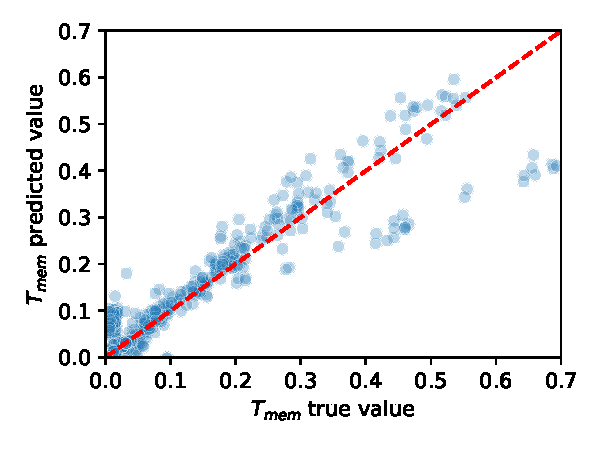
\includegraphics[width=0.5\linewidth]{chapters/05_cost_estimation/figures/analytical-regressor-fit.pdf}
    \caption{True $T_{mem}$ vs predicted $T_{mem}$ for the analytical estimator's $OperatorCost$ function. Tested on samples not used for training. MSE: $0.0295$.}
    \label{fig:5-analytical-regressor-fit}
\end{figure}

\subsection{Model-level Math and Memory cost}
\label{subsec:5-model-level-cost}
Here we describe the process of \textbf{calculating} the memory and math costs for each scenario. The memory cost is calculated as the total number of bytes read and written to memory divided by memory throughput. The math cost is calculated as the total number of FLOPs needed for a computation. These are the same definitions as used in the profiling experiments, however here we calculate them from the available data and model characteristics, instead of predicting them using a regressor, as was explained in the previous section.

The complexity of an operator or model was detailed previously. This complexity, or the number of Floating Point operations needed, is equal to the math costs and is calculated by inspecting the algorithms and summing the computations that are done. Various data characteristics such as the number of non-zero items and dataset sizes are taken into account in this process. For the memory costs we do the same, but we sum the number of bytes read and written to memory. For each ML model we add both the total summed costs as a feature, as well as the costs per involved operator. This results in numerous extra features that can be used to train the cost models.

A subset of the features is shown in \autoref{tab:5-feature-subset}. The full set of features is shown in \autoref{appendix:features}. The features are used to train the cost models, as detailed in the next section.

\begin{table}[ht]
    % LTeX: enabled=false
\begin{tabular}{llll}
\toprule
Dimension & Feature & Symbol & Formula \\
\midrule\midrule
\multirow[t]{5}{*}{Data} & Dataset size (rows, columns) & $r_T, c_T$ &  \\

 & Sparsity & $e_T$ & $\frac{nnz(T)}{r_T\times c_T}$ \\

 & Sparsity ratio &  & $\frac{e_T}{e_S}$ \\

 & Tuple ratio & $\tau$ & $\frac{\sum_{k=1}^p d_k}{d_S}$ \\

 & \# Base tables & $n$ &  \\
 
\multirow[t]{2}{*}{Data \& Model} & Complexity ratio &  & $\frac{FLOP_M}{FLOP_F}$ \\

 & Memory ratio &  & $\frac{\text{bytes}_M}{\text{bytes}_F}$ \\
 
\multirow[t]{2}{*}{Hardware} & Compute type &  &  \\

 & GPU memory bandwidth &  &  \\
 
\multirow[t]{2}{*}{Model} & Operator &  &  \\

 & \# Iterations & $iter$ &  \\
 
\multirow[t]{3}{*}{\textbf{Dependent}} & Execution Time & $\text{Time}_M$, $\text{Time}_F$ &  \\

 & Performance ratio &  & $\frac{\text{Time}_M}{\text{Time}_F}$ \\

 & Time saved &  & $\text{Time}_M - \text{Time}_F$ \\
 
\bottomrule
\end{tabular}

    \caption[Feature table]{Table showing a subset of the base, and derived/engineered features used for training the cost models}
    \label{tab:5-feature-subset}
\end{table}



\section{Cost Models}
\label{sec:5-cost-models}
\todo{Detail the full process going from data to Cost model, what features where used, and what is the inner architecture?\\Show each of the factors is significant. Data, Hardware, Model parameters.\\Show some score to compare between models.}

This section details the process of creating four different (types of) cost estimators capable of distinguishing when to use factorization over materialization. The estimators are created using the enriched dataset, as described in the previous section. The first estimator, which aims to be as explainable as possible, is an analytical estimator (\autoref{subsec:5-analytical}). Next we fit a variety of linear regressors to the dataset, to create a statistical estimator (\autoref{subsec:5-statistical}). The third estimator is a neural network, which is used to show the performance of a more complex model (\autoref{subsec:5-xgboost}). The last estimator is a hybrid model, which combines the analytical and statistical estimators to create a more accurate model. The performance of each of the models is evaluated on a validation set, and the results are shown in \autoref{subsec:5-comparing-performance}.



\subsection{Analytical}
\label{subsec:5-analytical}
\begin{figure}[ht]
    \centering
    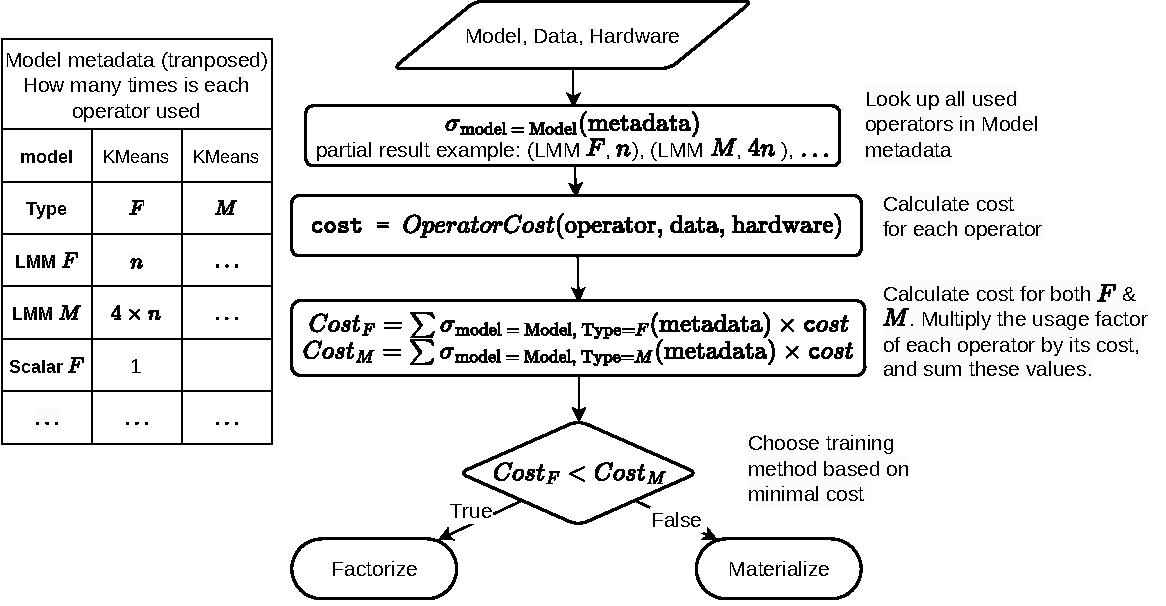
\includegraphics[width=\linewidth]{chapters/05_cost_estimation/figures/analytical-architecture.pdf}
    \caption[Analytical Estimator Architecture]{Architecture of the Analytical Estimator. Shows the control flow of inputs to a final decision on whether to use factorization or materialization. $OperatorCost$ is the function as defined in \autoref{fig:5-feature-enrichment}.}
    \label{fig:5-analytical-architecture}
\end{figure}
In \autoref{sec:5-gpu-performance-analysis} we have shown that the runtime of the evaluated ML scenarios is dominated by the time it takes to read from and to memory. To create an accurate prediction of the runtime of a scenario we can thus use the memory cost as a proxy, which is the approach taken with this analytical estimator. We evaluate two analytical estimators. The first estimator uses the collected profiling metrics to compute the memory cost of the factorized and materialized scenarios. The second uses the model-level memory cost introduced in \autoref{subsec:5-model-level-cost}.

\subsubsection{ANLY.1 Profiling Metrics Based Estimator}

The workflow for computing the factorized and materialized memory cost is shown in \autoref{fig:5-analytical-architecture}. We first collect the operators used for the model under test. We then use a regressor fit to the collected profiling metrics (as shown in \autoref{fig:5-feature-enrichment}) to predict the factorized and materialized operators' memory cost. This step is necessary as we do not have profiling metrics for the scenarios we are testing. Last, the costs for each training type are summed, and choose the scenario with the lowest predicted runtime.

A major downside of this estimator is that it requires a pre-trained regressor to predict the memory cost. This regressor is trained on a subset of the collected metrics, and is used to predict the missing metrics. The regressor we use is fit to a subset of factorized and materialized operator scenarios, so it is not fit to predict cost of operations that differ from the tested scenarios. Creating an estimator capable of predicting the memory cost for all scenarios is a complex task, and is left for future work.

\subsubsection{ANLY.2 Model-level Memory Cost Analysis Based Estimator}
By inspecting the operations performed during ML model training we can calculate the number of bytes read and written during computation. This is done by calculating the number of bytes read and written for each operation, and summing these values. The memory cost is then calculated by dividing the total number of bytes read and written by the memory throughput of the GPU. This estimator is easier to extend to novel ML models, as it does not require a pre-trained regressor to estimate operator cost. However, it does not take into account other factors that influence memory cost like cache layout and hit rates.

\subsubsection{Analytical Model Evaluation}
Both analytical estimators output a predicted memory cost for both the factorized and materialized case. To make the final decision we calculate the ratio between the cases and choose factorization if this ratio ($\frac{M}{F}$) is above some boundary. We then tune this boundary to reduce the number of false positives while still predicting factorization in those cases where it saves a lot of time over materialization. For ANLY.1 we set the boundary at $1.7$ and for ANLY.2 at $10.0$. The model only performing well with such a high ratio of materialized to factorized memory cost shows that a lot of overhead is added by using factorization in areas not reflected by this simple memory estimation.

The results of the evaluation are shown in \autoref{fig:5-analytical-model-evaluation}. Both models perform similarly well. The ANLY.1 model predicts a lot less false positives, but the sum of time lost by these false positives is almost the same as that of the FPs for ANLY.2. Subtracting the time lost for the FPs from the time saved for the true positives, we see that ANLY.2 saves more time than ANLY.1. This is likely due to the fact that ANLY.2 is more conservative in predicting factorization, and thus has a higher threshold for when to choose factorization over materialization. Altogether both models save around 250s of the total 1670s of the validation set. Breaking down the positively predicted cases by compute type we see that a lot of time (147s \& 136s respectively, shown in \autoref{fig:5-model-cpu-gpu}) is lost for false positives of CPU scenarios. So, for GPU scenarios the model is more accurate than for CPU scenarios, which is expected as we only use memory cost as an estimator for runtime. We have shown this to be a valid strategy for GPUs, but for CPUs the runtime is largely dominated by the number of FLOPs executed.

\begin{figure}[ht]
    \centering
    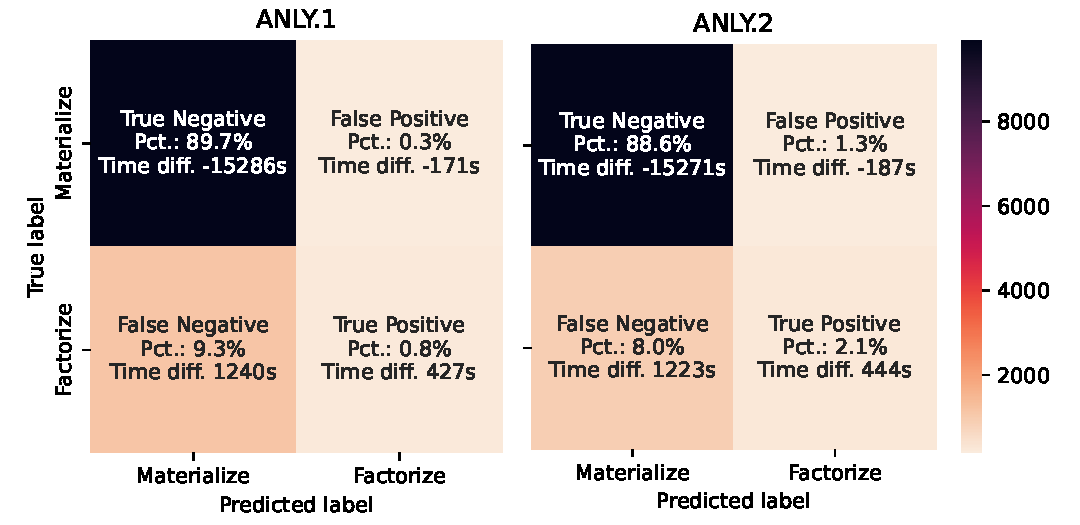
\includegraphics[width=0.9\linewidth]{chapters/05_cost_estimation/figures/analytical-models-compare.pdf}
    \caption[Analytical Model Confusion Matrix]{Confusion matrix of the analytical models' performance on the test set. Decision boundaries set at $1.7$ and $10.0$ respectively. Adding time difference of the false positive cases and the true positive cases gives the total time saved by the model. For ANLY.1 this is 256s, for ANLY.2 it is 257s. }
    \label{fig:5-analytical-model-evaluation}
\end{figure}


\subsection{Statistical}
\label{subsec:5-statistical}
The goal for this statistical estimator is to still be explainable, while providing higher performance than the hand tuned decision rules from related works. We use a variety of models, which all use linear regression at their core. We start with a singular regressor, and, by splitting the dataset by the categorical variables, end up at more complex models, with ensembles of linear regression models.

The architecture of each of the statistical models is shown in \autoref{fig:5-statistical-architecture}. In short, before training the dataset is split by a number of categorical variables (operator type, hardware type or $F$/$M$), or by filtering a part of the dataset. Each final model is a set of Linear Regression models, each fit to one of the subsets of the training data. For example, for STAT.3 we train two regressors. One on the factorization scenarios, and one on the materialization scenarios. During inference, each of the regressors is used to predict the runtime of the scenario under test. The output is the predicted materialized time minus the predicted factorized time. This is done to predict the time saved by choosing factorization over materialization. When a categorical variable is not used to split the dataset, it is used as a feature in the model.

\begin{figure}[ht]
    \centering
    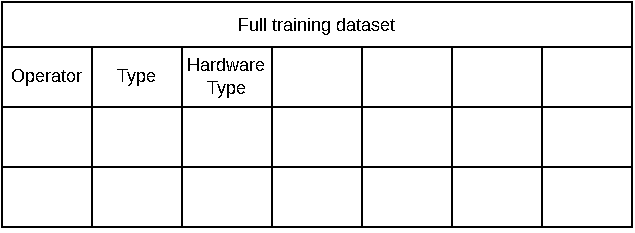
\includegraphics[width=\linewidth]{chapters/05_cost_estimation/figures/statistical-architecture.pdf}
    \caption[Statistical Estimator Architecture]{Architecture of the Statistical Estimators. Shows how the data, and estimators, are split for each model. The final split-level belonging to each respective model is coloured in the same colour. For STAT.5 we show the linear regression ensemble fit to the data. For clarity, we leave this out for the other models. Each box represents a regression model, the same-coloured boxes, connected via dotted lines, are combined into an ensemble to end up with the statistical cost estimators.}
    \label{fig:5-statistical-architecture}
\end{figure}

\subsubsection*{STAT.1 Linear Regressor Fit to Full Training Set}
The first linear regressor is trained on the full training set, which includes all operators. The rationale behind this approach is that there is likely a relationship between the performance of individual operators and the performance of the models in which they are used. By training the regressor on the full set of operators, we aim to capture these relationships and use them to improve the accuracy. This model predicts the time saved by choosing factorization over materialization.

\subsubsection*{STAT.2 Linear Regressor Fit to Model Runtimes}
The second linear regressor is trained on the runtimes of the models. With this model we find whether including the operators adds utility. Like STAT.1, this model predicts the time saved by choosing factorization over materialization.

\subsubsection*{STAT.3 Separate Regressors for F and M}
This model is an ensemble of two linear regressors, one for factorization and one for materialization. By training separate regressors for factorization and materialization, we aim to capture the relationships between independent variables and runtime more explicitly than is done by the previous models. Each internal regressor predicts the runtime of the scenario under test, and the final prediction is which is predicted to be faster.

\subsubsection*{STAT.4 Separate Regressors for each Model Type}
Much like STAT.3 this estimator is also a combination of multiple inner regressors. However, instead of having one regressor for each factorization and materialization, we have one regressor for each model type. This is done to capture the differences in the relationships between independent variables and runtime for different model types. Like the first two models, this model predicts the time saved by choosing factorization over materialization (by predicting whether time is saved by choosing F).

\subsubsection*{STAT.5 Separate Regressors for CPU and GPU}
In previous sections we have shown that the choice of hardware plays a large factor in the trade-off we are researching, therefore it is likely there are differences in the relationships between independent variables and runtime between CPU and GPU. A single linear regression model is likely unable to capture these differences. Therefore, we test the performance of a couple of estimators, one which is only fit to CPU scenario's, and one which is only fit to GPU scenario's.

\subsubsection*{STAT.6 Separate Regressors for F, M and Model Type}
The last version of the statistical model we created is a combination of STAT.4 and STAT.3. By training separate regressors for every combination of factorization, materialization and model type, we allow the models to capture differences between the groups more freely.

\subsubsection*{STAT.7 Separate Regressors For Each Combination of Categories}
The last, most granular, ensemble is one that has a separate regressor for each combination of factorization, materialization, model type and hardware. This is done to capture the differences in the relationships between independent variables and runtime for each combination of the dimensions.


\subsubsection{Statistical Model Evaluation}
\begin{figure}[ht]
    \centering
    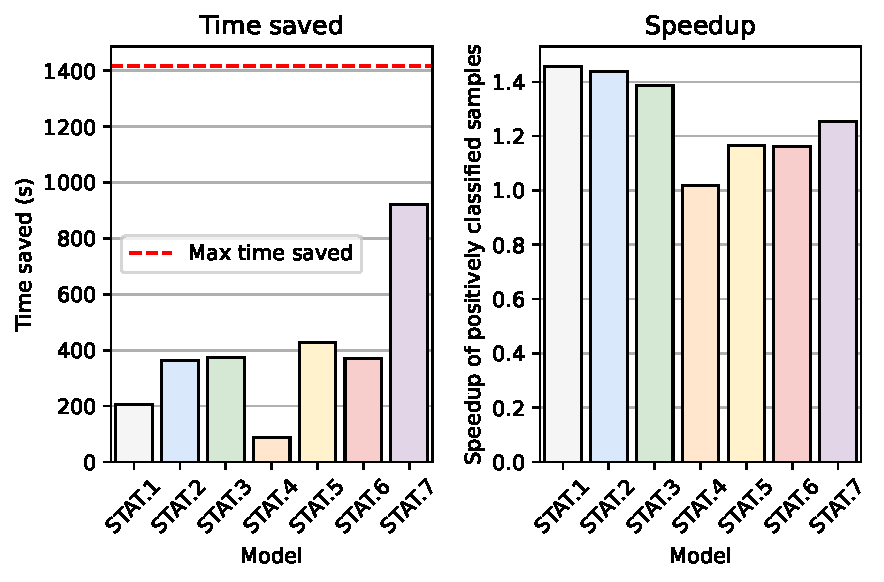
\includegraphics[width=0.75\linewidth]{chapters/05_cost_estimation/figures/stat-models-compare.pdf}
    \caption[Statistical Model Evaluation]{Evaluation of the statistical models on the validation set (synthetic data, only models). The plots show statistics of those scenarios where the estimator predicts factorization to be faster. }
    \label{fig:5-statistical-model-evaluation}
\end{figure}

A performance comparison for the statistical models is shown in \autoref{fig:5-statistical-model-evaluation}. We choose to highlight the cases where the model predicts factorization to be faster, and evaluate the saved time in these cases. Overall, estimators that fit more distinct regressors perform better, showing that each of the chosen categorical variables has impact on the F/M trade-off.

STAT.1-3 show relatively little time saved, but the average speedup of positively classified cases is high. This is due to these models producing either producing a lot of false negatives, missing out on a lot of time saved (STAT.1), or a lot of false positives, which drags down the total time saved (STAT.2,3). STAT.4, split only by model type performs worst of the estimators showing that there is a relation for the speedup between the different model types. Estimators STAT.5,6 both find a relatively large fraction of the positive samples, at the cost of a lot of false positives and negatives. STAT.7, which is the most granular, performs best on the validation set. This is likely due to the fact that it can capture the differences in the relationships between independent variables and runtime for each combination of the dimensions. This estimator is the most complex, but also the most accurate, performing 65\% as well as a perfect cost model would, when looking at the time saved.

However, when evaluating on the test datasets, the performance of the models is much lower. This is likely due to the fact that the models are overfitting to the training data (which only contains synthetic dataset scenarios). Only the models STAT.1 and STAT.5 perform relatively well, which can be explained by the fact that they do not use extensive partitioning of the training data, preventing the regression from fitting to the training data. To solve this overfitting we choose to evaluate the performance of a more complex model.

\subsection{XGBoost}
\label{subsec:5-xgboost}
The third model type we evaluate is XGBoost \cite{xgboost}, specifically an \texttt{XGBRegressor}\footnote{\url{https://xgboost.readthedocs.io/en/stable/python/python_api.html\#xgboost.XGBRegressor}}. This model is a gradient boosting algorithm, which is an ensemble learning method, using a series of decision trees. We use XGBoost as it has shown excellent performance in related cost prediction scenarios \cite{tvm}, as well as showcasing excellent ability for handling unbalanced datasets \cite{xgboost_imbalanced_data}. The model is trained on the same dataset as the statistical models, and uses the same features.

\begin{table}[ht]
    \centering
    \begin{tabular}{llll}
        \toprule
        Model & Target     & Pruning       & Decision Boundary            \\
        \midrule \midrule
        XGB.1 & Runtime    & All operators & $Time_M > Time_F$            \\
        XGB.2 & Runtime    & Only models   &                              \\
        XGB.3 & Speedup    & All operators & $\texttt{speedup} > 1.0$     \\
        XGB.4 & Speedup    & Only model    &                              \\
        XGB.5 & Time saved & All operators & $\texttt{time\_saved} > 0.0$ \\
        XGB.6 & Time saved & Only models   &                              \\
        \bottomrule
    \end{tabular}
    \caption[XGBoost configurations]{Overview of the different configurations for the XGBoost models.}
    \label{tab:5-xgboost-configurations}
\end{table}

We explore a number of different configurations for this model. The models differ along two axes: their target variable, and whether all operators are included, or just the model operators, in the training dataset. The target variable can be the runtime of the scenario (one target for factorized, one for materialized), the speedup of a scenario, or the time saved by choosing factorization over materialization. The dataset can be pruned only keeping training samples where the operator is one of the model types (K-Means, Logistic Regression, Linear Regression, or GNMF), or keeping all samples. By evaluating multiple models with different configurations, we aim to find the model that best captures the relationships between independent variables and the F/M trade-off. The overview of which model uses which configuration, and how the decision to materialize or factorize is made based on the predicted value(s), is shown in \autoref{tab:5-xgboost-configurations}.

\begin{figure}[ht]
    \centering
    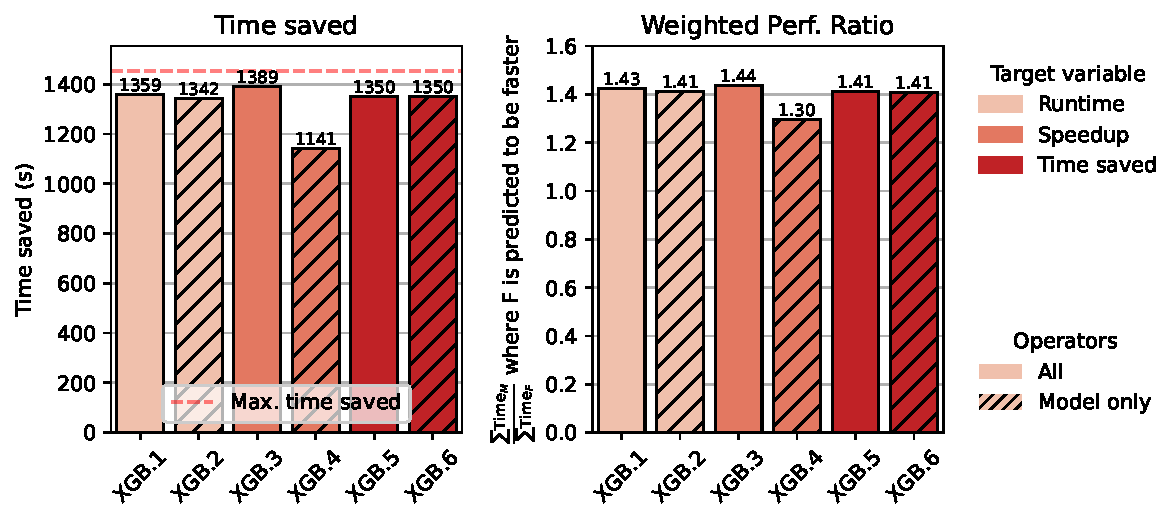
\includegraphics[width=\linewidth]{chapters/05_cost_estimation/figures/xgb-models-compare.pdf}
    \caption[XGBoost Estimator Comparison]{Evaluation of the XGBoost models on the validation set.}
    \label{fig:5-xgboost-evaluation}
\end{figure}

A comparison and evaluation of the XGB models is shown in \autoref{fig:5-xgboost-evaluation}. As expected, as these models are more complex, they perform better than the statistical models. Amongst the XGB models there is little difference in performance on the validation set. There is no significant difference between which target variable is used, or whether all operators are used in the training set. XGB.3, which predicts the speedup of factorization over materialization, barely outperforms the other models, predicting 98\% of the validation scenarios correctly.

\todo{Evaluate Feature importances.}

\subsection{Comparing Performance}
\label{subsec:5-comparing-performance}
The performance of the two best estimators per type is shown in \autoref{fig:5-model-cpu-gpu}. We show the total time saved on the test scenarios, which includes the scenarios on Hamlet and TPCx-AI datasets. As expected, the least explainable, most complex, XGBoost models perform best. XGB.3 and XGB.5 respectively save $600$ and $700$ seconds of the total $1670$ seconds. The statistical model performs worst, likely due to overfitting to the synthetic data in the training set. Interesting, however, is splitting the performance by compute type. The XGBoost models perform drastically better on GPU scenarios than on CPU scenarios, whereas STAT.5 performs better on CPU scenarios. This is due to the fact that STAT.5 consists of two separate regressors, one for CPU and one for GPU, which allows it to capture the differences in the relationships between independent variables and runtime for each compute type. How these models are combined to create a more accurate hybrid model is covered next.

\begin{figure}[ht]
    \centering
    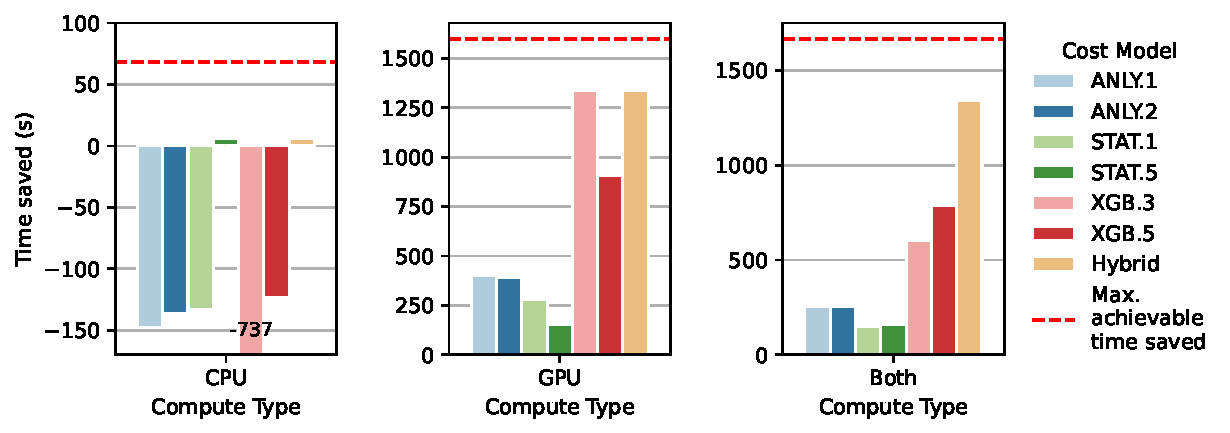
\includegraphics[width=0.9\linewidth]{chapters/05_cost_estimation/figures/compare_gpu_vs_cpu.pdf}
    \caption[Cost Model Comparison Broken Down by Compute Type]{Comparison of the best models, broken down by compute type. Evaluated on the test set.}
    \label{fig:5-model-cpu-gpu}
\end{figure}

\subsubsection{Combining Cost Models}
\label{subsec:5-hybrid}
To create the final cost model we combine the best of the models. We use the XGBoost model for GPU scenarios, and the STAT.5 model for CPU scenarios. This is done to capture the differences in the relationships between independent variables and runtime for each compute type. The final model is evaluated on the test set, and the results are shown in \autoref{fig:5-hybrid-model-evaluation}. The model achieves 80\% of the performance of a perfect cost model, saving 1344 seconds of the total 1670 seconds. This is a significant improvement over the best individual models, which achieved a maximum of 47\% of theoretical performance.

\subsubsection{Meta-results}
In the ML framework proposed in \cite{amalur}, which this thesis creates a cost model for, the decision between factorization and materialization is made at runtime, and should therefore not introduce any overhead to the training process. We briefly discuss the overhead introduced by the cost of inference of the models, as well as other factors that can affect the choice between cost models. The overview of all facets is shown in \autoref{tab:5-meta-results}.

The first facet we discuss is training time, which is very fast for statistical models, but slower for the XGBoost model. The outliers in this case are the analytical models. ANLY.1 is extremely slow as it needs to fit a large set of regressors, one for each combination of operator and F/M. ANLY.2, on the other hand, does not have training time in the traditional sense as it uses a handcrafted formula. As for Extensibility the ANLY.1 models are easiest to extend for new ML models, as they already have an underlying “understanding” of the used operators. For the remaining models an updated training set is needed which includes the new ML models. Arguably the most important factor, other than performance, is inference speed, as we do not want overhead in the training process. ANLY.2 and Statistical model are very quick as they are a simple equation with no more than $30$ terms. XGBoost, and thus the hybrid model, is slightly slower, but still quick. ANLY.1 is slowest here, as computing the $OperatorCost$ of all involved operators is costly. The last facet is performance, which is discussed in the previous section.

\begin{table}[ht]
    \centering
    \begin{tabular}{lllll}
        \toprule
        Model        & Training time & Extensibility & Inference Speed & Performance \\
        \midrule
        Analytical 1 & Slow          & Easy          & Slow            & Bad         \\
        Analytical 2 & --            & Easy          & Quick           & Bad         \\
        Statistical  & Fast          & Difficult     & Quick           & Bad         \\
        XGBoost      & Medium        & Difficult     & Medium          & Mediocre    \\
        Hybrid       & Medium        & Difficult     & Medium          & Good        \\
        \bottomrule
    \end{tabular}
    \caption{Comparison of the different models.}
    \label{tab:5-meta-results}
\end{table}



